% TdeGPAE es el archivo principal para construir el Trabajo de Grado en Estad\'{\i}stica en la Universidad del Valle
% EncabezadoPAE load packages to TdeGPAE

\documentclass[12pt,fleqn,openany,letterpaper]{book} %draft option

\usepackage[english]{babel}
\usepackage[utf8]{inputenc}
%\usepackage{fancyhdr}
\usepackage{graphicx,epsfig}
\usepackage{amsmath}
\usepackage{amssymb}
\usepackage{natbib}
\usepackage{tabularx}
\usepackage{longtable}
%\usepackage{hyperref}
%\usepackage{url}
\usepackage{kpfonts}

%\usepackage[none]{hyphenat}
%    \sloppy

\usepackage{ragged2e}
	\justifying

\renewcommand{\theequation}{\thechapter-\arabic{equation}}
\renewcommand{\thefigure}{\textbf{\thechapter-\arabic{figure}}}
\renewcommand{\thetable}{\textbf{\thechapter-\arabic{table}}}

%\pagestyle{fancyplain}
\textheight20.5cm
%\topmargin0cm
\textwidth16.5cm
\oddsidemargin0.5cm
\evensidemargin-0.5cm

%\setlength{\headheight}{15pt}

%\renewcommand{\chaptermark}[1]{\markboth{\thechapter\; #1}{}}
%\renewcommand{\sectionmark}[1]{\markright{\thesection\; #1}}
%\lhead[\fancyplain{}{\thepage}]{\fancyplain{}{\rightmark}}
%\rhead[\fancyplain{}{\leftmark}]{\fancyplain{}{\thepage}}
%\fancyfoot{}
%\thispagestyle{fancy}

%\addtolength{\headwidth}{0cm}
\unitlength1mm %Define la unidad LE para Figuras
\mathindent0cm %Define la distancia de las formulas al texto,  fleqn las descentra
%\marginparwidth0cm
\parindent0cm %Define la distancia de la primera linea de un parrafo a la margen

%Espacio entre lineas
\renewcommand{\baselinestretch}{1.1}

%El includeonly sirve para compilar y trabajar s\'{o}lo en la secci\'{o}n seleccionada. Por ejemplo, si dejamos la instucci\'{o}n siguiente, el sistema s\'{o}lo compilar\'{a} los caps\'{\i}tulos 2 y 3.
%\includeonly{Kap2/Cap2,Kap3/Cap3}

\begin{document}
\pagenumbering{roman}

% HojaTituloPAE contiene toda la informaci\'{o} acerca de la presentaci\'{o}n del Trabajo de Grado
\thispagestyle{empty}

\begin{center}
\begin{figure}
\centering

\epsfig{file=HojaTitulo/Fig_HojaTitulo/Univalle.jpg,scale=0.15}
\end{figure}\vspace*{2.0cm}

%Reemplace este t\'{\i}tulo por el de su Trabajo de Grado
\textbf{\huge Procesos estocásticos irregularmente espaciados}\vspace*{4.0cm}

%Aqui va los nombres y apellidos completos de los autores
\Large\textbf{Wilmar Sepulveda Herrera}\vspace*{4.0cm}

\small Universidad del valle

Facultad de Ingeniería, Escuela de Estadística

Cali, Valle del Cauca

%Modifique fecha de ser necesario
2022
\end{center}

\newpage{\pagestyle{empty}\cleardoublepage}

\newpage

\thispagestyle{empty}

\begin{center}
%Reemplace este t\'{\i}tulo por el de su Trabajo de Grado
\textbf{\huge Procesos estocásticos irregularmente espaciados}\vspace*{1.0cm}

by\vspace*{0.5cm}

%Aqui va los nombres y apellidos completos de los autores
\Large\textbf{Wilmar Sepulveda Herrera}\vspace*{1.0cm}

\small Trabajo de investigación para optar por el título de:\vspace*{1.0cm}

%Modifique seg\'{u}n el g\'{e}nero
\textbf{Magister en}\vspace*{0.5cm}

En\vspace*{0.5cm}

\textbf{Estadística}\vspace*{1.5cm}

Aceptamos esta tesis\\
Conforme a los requerimientos de la norma\vspace*{1.0cm}

\rule{10cm}{1pt}\vspace*{0.7cm}
\rule{10cm}{1pt}\vspace*{0.7cm}
\rule{10cm}{1pt}\vspace*{2.3cm}

\small Universidad del valle

Facultad de Ingeniería, Escuela de Estadística

Cali, Valle del Cauca

%Modifique fecha de ser necesario
2022
\end{center}

\newpage

\thispagestyle{empty}

\vspace*{1cm}

\textbf{\LARGE Dedicatoria}\vspace*{4.0cm}

\begin{flushright}
\begin{minipage}{8cm}
A mi familia.
\end{minipage}
\end{flushright}

\newpage{\pagestyle{empty}\cleardoublepage}

\newpage

\thispagestyle{empty}

\vspace*{1cm}

\textbf{\LARGE Agradecimientos}\vspace*{1.0cm}

Estoy agradecido con\ldots

\newpage{\pagestyle{empty}\cleardoublepage}

\newpage

\vspace*{1cm}

\textbf{\LARGE Abstract}\vspace*{1cm}
\addcontentsline{toc}{chapter}{\numberline{}Abstract}

El resumen es una presentaci\'{o}n abreviada y precisa. Se debe usar una extensi\'{o}n m\'{a}xima de 12 renglones. Se recomienda que este resumen sea anal\'{\i}tico, es decir, que sea completo, con informaci\'{o}n cuantitativa y cualitativa, generalmente incluyendo los siguientes aspectos: objetivos, dise\~{n}o, lugar y circunstancias (u objetivo del estudio), principales resultados, y conclusiones. Al final del resumen se deben usar palabras claves tomadas del texto (m\'{\i}nimo 3 y m\'{a}ximo 7 palabras), las cuales permiten la recuperaci\'{o}n de la informaci\'{o}n.\vspace*{0.5cm}

\textbf{\small Palabras clave: palabras clave en espa\~{n}ol (m\'{a}ximo 10 palabras, preferiblemente seleccionadas de las listas internacionales que permitan el indizado cruzado)}\vspace*{1cm}

\textbf{\LARGE Resumen}\vspace*{1cm}

Es el mismo resumen pero traducido al ingl\'{e}s. Se debe usar una extensi\'{o}n m\'{a}xima de 12 renglones. Al final del Abstract se deben traducir las anteriores palabras clave tomadas del texto (m\'{\i}nimo 3 y m\'{a}ximo 7 palabras), llamadas keywords. Es posible incluir el resumen en otro idioma diferente al espa\~{n}ol o al ingl\'{e}s, si se considera como importante dentro del tema tratado en la investigaci\'{o}n, por ejemplo: un trabajo dedicado a problemas ling\"{u}\'{\i}sticos del mandar\'{\i}n seguramente estar\'{\i}a mejor con un resumen en mandar\'{\i}n.\vspace*{0.5cm}

\textbf{\small Keywords: palabras clave en ingl\'{e}s (m\'{a}ximo 10 palabras, preferiblemente seleccionadas de las listas internacionales que permitan el indizado cruzado)}

\newpage{\pagestyle{empty}\cleardoublepage}

%\renewcommand{\tablename}{\textbf{Tabla}}
%\renewcommand{\figurename}{\textbf{Figura}}
%\renewcommand{\listtablename}{Lista de Tablas}
%\renewcommand{\listfigurename}{Lista de Figuras}
%\renewcommand{\contentsname}{Contenido}
\renewcommand{\bibname}{References}

\tableofcontents

\listoffigures
\addcontentsline{toc}{chapter}{\numberline{}List of figures}

\listoftables
\addcontentsline{toc}{chapter}{\numberline{}List of tables}

%%Se incluyen s\'{\i}mbolos generales (con letras latinas y griegas), sub\'{\i}ndices, super\'{\i}ndices y abreviaturas (incluir s\'{o}lo las clases de s\'{\i}mbolos que se utilicen). Cada una de estas listas debe estar ubicada en orden alfab\'{e}tico de acuerdo con la primera letra del s\'{\i}mbolo.

\chapter*{Lista de s\'{\i}mbolos}
{\textbf{\LARGE}
\addcontentsline{toc}{chapter}{\numberline{}Lista de s\'{\i}mbolos}}

\section*{S\'{\i}mbolos con letras latinas} \label{simbolos}
\renewcommand{\arraystretch}{1.3}

\begin{longtable}[l]{>{$}l<{$}l>{$}l<{$}>{$}l<{$}}
\textbf{S\'{\i}mbolo} & \textbf{T\'{e}rmino} & \textbf{Definici\'{o}n} \\ [0.5ex] \hline
\endfirsthead
\textbf{S\'{\i}mbolo} & \textbf{T\'{e}rmino} & \textbf{Definici\'{o}n} \\ [0.5ex] \hline
\endhead
w & Periodo de garant\'{\i}a  & \text{Miles de horas de garant\'{\i}a} \\
k & Subconjunto de las componentes del sistema & \text{Componentes necesarias} \\
 & & \text{para que el sistema funcione} \\
n & N\'{u}mero de componentes del sistema & \\
T^{II} & Tiempo de vida del sistema bajo & \text{N\'{u}mero de horas que transcurren hasta} \\
 & aproximaci\'{o}n de caja negra & \text{que el sistema presenta falla tipo II} \\
Z_{w}^{FRW} & Proceso de costo pol\'{\i}tica FRW & \\
Z_{w}^{PRW} & Proceso de costo pol\'{\i}tica PRW & \\
\end{longtable}

\vspace{5ex}

\setlength{\extrarowheight}{0pt}

\section*{S\'{\i}mbolos con letras griegas} \label{simbolosg}

\begin{longtable}[l]{>{$}l<{$}l>{$}l<{$}>{$}l<{$}}
\textbf{S\'{\i}mbolo} & \textbf{T\'{e}rmino} & \textbf{Definici\'{o}n} \\ [0.5ex] \hline
\endfirsthead
\textbf{S\'{\i}mbolo} & \textbf{T\'{e}rmino} & \textbf{Definici\'{o}n} \\ [0.5ex] \hline
\endhead
\lambda^{j}(\cdot) & \text{Tasa de falla} & \text{Tasa de falla del sistema} \\
 & & \text{debido a la falla $ j=1,2 $} \\
\zeta & \text{Tiempo de vida del sistema} & \text{N\'{u}mero de horas que transcurren hasta que un} \\
 & \text{bajo aproximaci\'{o}n f\'{\i}sica} & \text{componente cr\'{\i}tico presenta falla de tipo II} \\
\eta & \text{N\'{u}mero de renovaciones} & \text{N\'{u}mero de renovaciones del sistema dentro} \\
 & & \text{de la garant\'{\i}a} \\
\end{longtable}

\setlength{\extrarowheight}{0pt}

%\section*{Sub\'{\i}ndices} \label{subindices}
%\renewcommand{\arraystretch}{1.4}

%\begin{longtable}[l]{>{}l<{}l}
%\textbf{Sub\'{\i}ndice} & \textbf{T\'{e}rmino} \\ [0.5ex] \hline
%\endfirsthead
%\textbf{Sub\'{\i}ndice} & \textbf{T\'{e}rmino} \\ [0.5ex] \hline
%\endhead
%bm & Materia org\'{a}nica \\
%DR & Dubinin-Radushkevich \\
%E & Experimental \\
%g & Fase gaseosa \\
%k & Condensado \\
%Ma & Macroporos \\
%P & Part\'{\i}cula \\
%p & Poro \\
%p & Pirolizado \\
%R & Reacci\'{o}n \\
%t & Total \\
%wf & Libre de agua \\
%waf & Libre de agua y de ceniza \\
%0 & Estado de referencia \\
%\end{longtable}

%\setlength{\extrarowheight}{0pt}

%\section*{Super\'{\i}ndices} \label{superindices}
%\renewcommand{\arraystretch}{1.4}

%\begin{longtable}[l]{>{}l<{}l}
%\textbf{Super\'{\i}ndice} & \textbf{T\'{e}rmino} \\ [0.5ex] \hline
%\endfirsthead
%\textbf{Super\'{\i}ndice} & \textbf{T\'{e}rmino} \\ [0.5ex] \hline
%\endhead
%n & Coeficiente x \\
%\end{longtable}

%\setlength{\extrarowheight}{0pt}
\newpage

\section*{Abreviaturas} \label{abreviaturas}
\renewcommand{\arraystretch}{1.4}

\begin{longtable}[l]{>{}l<{}l}
\textbf{Abreviatura} & \textbf{T\'{e}rmino} \\ [0.5ex] \hline
\endfirsthead
\textbf{Abreviatura} & \textbf{T\'{e}rmino} \\ [0.5ex] \hline
\endhead
$FRW$ & Pol\'{\i}tica de garant\'{\i}a de sustituci\'{o}n o reparo gratuito para el consumidor \\
$PRW$ & Pol\'{\i}tica de garant\'{\i}a de sustituci\'{o}n o reparo pro-rata para el consumidor \\
$c.d.f$ & Funci\'{o}n de distribuci\'{o}n \\
$p.d.f$ & Funci\'{o}n de densidad \\
\end{longtable}

\setlength{\extrarowheight}{0pt} https://www.dickimaw-books.com/latex/thesis/html/makeglossaries.html
\pagenumbering{arabic}
\chapter{Introducci\'{o}n}
En la introducci\'{o}n, \citep{Harvard:2008} el autor presenta y se\~{n}ala la importancia, el origen (los antecedentes te\'{o}ricos y pr\'{a}cticos), los objetivos, los alcances, las limitaciones, la metodolog\'{\i}a empleada, el significado que el estudio tiene en el avance del campo respectivo y su aplicaci\'{o}n en el \'{a}rea investigada. No debe confundirse con el resumen y se recomienda que la introducci\'{o}n tenga una extensi\'{o}n de m\'{\i}nimo 2 p\'{a}ginas y m\'{a}ximo de 4 p\'{a}ginas.
\chapter{Marco teórico}
Para el tratamiento de procesos estocásticos y series de tiempo, ha sido mucha la teoría estadística implementada y se ha convertido
en una herramienta importante para tratar observaciones dependientes y entender la naturaleza de dicha dependencia,
la mayoría de estos métodos, asumen que las series de timpo son regulamente espaciadas, sin embargo este escenario
no siempre se da y ahi es donde cobran importancia los procesos estocásticos irregularmente espaciados.

Este capitulo tiene la siguiente estructura, en la seccción 2.1 presentamos la definición matematica de un proceso
estocastico irregularmente espaciado. En la sección 2.2 se presenta un proceso estocástico autorregresivo irregulamente
espaciado. En la sección 2.3 se presenta un proceso estocástico irregularmente espaciado de medias moviles y en la sección
2.3 se presenta un proceso estocástico atorregresivo de medias moviles irregulamente espaciado.


\section{Procesos estocásticos irregularmente espaciados}
Sea $(\Omega,\mathscr{B},P)$ un espacio de probabilidad. Si se define un proceso estocástico como una medida 
que mapea $x: \Omega \mapsto \mathbb{R}^{\mathbb{T}}$, donde 

$$x(\omega)= \lbrace X_{\tau}(\omega), \tau \in \mathbb{T}\rbrace$$

$\mathbb{T}$ es llamado conjunto de índices y la variable aleatoria $X_{\tau}(\omega)$ es llamada coordenada 
del proceso o trayectoria. Consideremos ahora $\mathbb{T}'= \lbrace t_1,t_2, t_3,... \rbrace$, 
con $\Delta_{n+1}=t_{n+1}-t_{n}$, para $n\geq 1$

$$x'= \lbrace X_{\tau}(\omega), \tau \in \mathbb{T}'\rbrace$$

$x'$ es un proceso estocástico irregularmente espaciado. Una serie de tiempo irregularmente espaciada es una 
realización finita de un proceso estocástico irregularmente espaciado. Note que si  $\Delta_{n+1}=t_{n+1}-t_{n}=1$ 
para $n \geq 1$, el proceso $x'$ es un proceso regularmente espaciado, por tanto esta definición es más general.

\section{Formas de describir un proceso estocástico}
Una forma de describir un proceso estocástico $x$, es especificar la función de distribución conjunta de 
$\lbrace X_{\tau_1},X_{\tau_2}, ..., X_{\tau_n}\rbrace$ para todo $n$, este es llamado 
\emph{punto de vista distribucional}. Por otra parte, se puede describir el proceso proporcionando 
una formula para el valor $X_{\tau}$ para cada punto $\tau$ en términos de una familia de variables aleatorias 
con comportamiento probabilístico conocido, esto hace que podamos ver el proceso como una función de otros 
procesos (o cómo familias de procesos iid); esta forma es llamada \emph{punto de vista construccionista}.

\section{El proceso de medias móviles irregular de primer orden (IMA)}
Teniendo en cuenta el conjunto $\mathbb{T}'= \lbrace t_1,t_2, t_3,... \rbrace$ propuesto anteriormente, 
tal que sus diferencias $\Delta_{n+1}$ para $n\geq 1$ están acotados uniformemente lejos de cero. Ahora, 
sea $m: \mathbb{T}' \mapsto \mathbb{R} $ una función tal que $m(t_n)=0$, para cualquier $t_n \in \mathbb{T}'$. 
A continuación, sea $\Gamma: \mathbb{T}'x\mathbb{T}' \mapsto \mathbb{R}$ una función tal que para cualquier 
pareja $t_n,t_s \in \mathbb{T}'$,

\begin{equation*}
\Gamma (t_n,t_s)=
    \begin{cases}
    \gamma_0& |n-s|=0\\
    \gamma_1,\Delta_{max(n,s)} & |n-s|=1\\
    0 & |n-s|\geq1\\
    \end{cases}
\end{equation*}

Note que $\Gamma$ puede ser representada cómo una matriz diagonal así

\begin{equation}
    \Gamma=
	\begin{bmatrix} 
	\gamma_0 & \gamma_1,\Delta_2 & 0 & 0 & ... \\
	\gamma_1,\Delta_2 & \gamma_0 & \gamma_1,\Delta_3 & 0\\
	0 & \gamma_1,\Delta_3 & \gamma_0 & \gamma_1,\Delta_4 \\
	.& & & & . \\
	.& & & & & .\\
	. & & & & & & .
	\end{bmatrix}
	\quad
	\label{mat1}
\end{equation}

Ser $\Gamma_n$ la truncacion $nxn$ de $\Gamma$ y asumiendo $\gamma_1,\Delta_j\neq 0$, para $j=2,...n$, $\Gamma_n$ 
es definida positiva si $\gamma_0$ y $(\frac{\gamma_1,\Delta_{n+1}}{\gamma_0})^2 \leq 1/4$, para $j=2,...,n$

Esto implica que existe un proceso Gaussiano estacionario $\lbrace X_{t_n},t_n, \tau \in \mathbb{T}\rbrace$, 
único hasta la equivalencia, con media 0 y covarianza $\Gamma$. Este proceso es llamado, proceso de medias móviles
 de primer orden irregularmente espaciado de forma general. A continuación se darán las expresiones particulares 
 de este proceso desde los dos puntos de vista antes definidos.

\subsubsection{El punto de vista distribucional}
En (\ref{mat1}), $\gamma_0$ y $\gamma_{1,\Delta_{n+1}}$, para $n\geq1$, representa la varianza y las covarianzas 
de primer orden respectivamente. Definimos la varianza cómo $\gamma_0=\sigma^2(1+\theta^2)$ y las covarianzas de 
primer orden cómo $\gamma_{1,\Delta_{n+1}}=\sigma^2 \theta^{\Delta_{n+1}}$, $\sigma^2 >0$ y $0<\theta <1$. 
Por tanto, obtenemos el proceso estocástico irregularmente espaciado de primer orden con matriz de covarianzas

\begin{equation}
    \Gamma=
	\begin{bmatrix} 
	1+\theta^2 & \theta^{\Delta_2} & 0 & 0 & ... \\
	\theta^{\Delta_2} & 1+\theta^2 & \theta^{\Delta_3}& 0\\
	0 & \theta^{\Delta_3} & 1+\theta^2 & \theta^{\Delta_4} \\
	.& & & & . \\
	.& & & & & .\\
	. & & & & & & .
	\end{bmatrix}
	\quad
	\label{mat2}
\end{equation}

el cual contiene el modelo de medias moviles convencional cómo caso especial. Este es llamado proceso Gaussiano 
irregular de medias moviles de primer orden.

\subsubsection{El punto de vista construccionista}
Ahora, cómo es usual, especificaremos el proceso IMA cómo función de otros procesos estocásticos. 
Sea $\lbrace \epsilon_{t_n}\rbrace n\geq 1$ variables aleatorias independientes que siguen una distribución 
normal $N(0,\sigma^2 c_n(\theta))$ con $\sigma^2 >0, 0<\theta<1, c_1(\theta)=1+\theta^2$ y

$$
c_n(\theta)=1+\theta^2-\frac{\theta^{2\Delta_n}}{c_{n-1}(\theta)} para, n\geq 2
$$

donde $\Delta_n=t_n-t_{n-1}$. El proceso $\lbrace X_{t_n},t_n \in \mathbb{T'} \rbrace$, es decirse tiene un proceso 
IMA si $X_{t_1}=\epsilon_{t_1}$ y para $n\geq 2 $

\begin{equation}
    X_{t_n}= \epsilon_{t_n}+\frac{\theta^{\Delta_n}}{c_{n-1}(\theta)}\epsilon_{t_{n-1}}
\end{equation}
Decimos que $\lbrace X_{t_n},t_n \in \mathbb{T'} \rbrace$ es un proceso IMA con media 
$\mu$ si $\lbrace X_{t_n}-\mu,t_n \in \mathbb{T'} \rbrace$ es un proceso IMA


Cambiando el marco teorico en rama, hola mamamamamam
ssjsjsjsj nuevamente cambio el marco

estoy subiendo esto al remoto
\chapter{Bibliograf\'{\i}a, Figuras, Tablas y Ecuaciones}

La Norma T\'{e}cnica Colombiana NTC 1486 fija la reglamentaci\'{o}n nacional para la ``presentaci\'{o}n de tesis, trabajos de grado y otros trabajos de investigaci\'{o}n'' \citep{NTC1486}. Se recomienda a los autores revisar cuidadosamente la Norma para familiarizarse con su contenido antes de empezar a escribir su propio documento. Pero adem\'{a}s, se recomienda mantener el documento a mano como fuente de referencia permanente. \\

Por otra parte, la Norma T\'{e}cnica Colombiana NTC 5613 se refiere a las referencia bibliogr\'{a}ficas, su contenido, forma y estructura \citep{NTC5613}. En esta plantilla se recogen las ideas generales de la Norma NTC 5613, para lo cual se utiliza el estilo de citas \emph{agsm} (tipo autor-a\~{n}o), tomado de la familia de estilos bibliogr\'{a}ficos \emph{Harvard} \citep{Harvard:2008}, pero usando el paquete de referencias y citas para las ciencias naturales \emph{Natbib} \citep{Natbib:2010, Natbib:2010RS}. \\

Las figuras, tablas y ecuaciones se enumeran consecutivamente dentro de cada cap\'{\i}tulo. \\

Las siguientes secciones de este cap\'{\i}tulo describen c\'{o}mo citar las referencias bibliogr\'{a}ficas y como referenciar en el texto las figuras, las tablas y las ecuaciones.

\section{Citas bibliogr\'{a}ficas}

En primer lugar, se debe crear un archivo con todas las referencias bibliogr\'{a}ficas. En esta plantilla este archivo tiene la extensi\'{o}n \emph{bib} y se llama \emph{BiblioPAE}. Los archivos tipo \emph{bib} tienen entradas que el programa {\textsc{Bib}}{\TeX} interpreta e incorpora en el documento final. \\

Por ejemplo, la cita del trabajo \citet{Harvard:2008} se introduce en el archivo BiblioPAE.bib de la siguiente manera:

\begin{verbatim}
	@Manual{Harvard:2008,
	title = {The {H}arvard {F}amily of {B}ibliography {S}tyles},
	author = {Peter Williams and Thorsten Schnier},
	month = {Noviembre},
	year = {2008},
	note = {ftp://ftp.tex.ac.uk/tex-archive/macros/latex/contrib/harvard/harvard.pdf},
}
\end{verbatim}

Dependiendo de la forma en que se introduzca la cita, \'{e}sta lucir\'{a} de manera diferente. Por ejemplo, si se usa
\verb"\citet{Harvard:2008}", la referencia ser\'{a}  adecuada para una expresi\'{o}n de la forma: ``... de acuerdo con \citet{Harvard:2008}...'' \\

Pero si se usa
\verb"\citep{Harvard:2008}", la referencia ser\'{a} m\'{a}s adecuada para la expresi\'{o}n: ``... si se usa el estilo \emph{Harvard} \citep{Harvard:2008}...'' \\

Para otras variaciones de la forma de citar, consulte el manual de \emph{Natbib} \citep{Natbib:2010}. \\

Los siguientes ejemplos pueden resultar \'{u}tiles para ilustrar la forma de citar en el documento:

\begin{itemize}

\item El sistema de procesamiento estad\'{\i}stico de libre distribuci\'{o}n \emph{\textbf{R}} \citep{R} se utiliza para ejecutar el procesamiento de los datos en este Trabajo de Grado.

\item En este Trabajo de Grado se utiliza la librer\'{\i}a Lattice de \emph{\textbf{R}} \citep[ver][]{Sarkar:2008}.

\item Seg\'{u}n \citet{Wood:2003}, la suavizaci\'{o}n spline es una de las t\'{e}cnicas m\'{a}s comunes para estimar la funci\'{o}n de regresi\'{o}n en los m\'{e}todos de regresi\'{o}n no param\'{e}trica.

\item El modelo de regresi\'{o}n lineal podr\'{\i}a considerarse el m\'{e}todo estad\'{\i}stico m\'{a}s utilizado en el an\'{a}lisis de datos \citep{Graybill:1976, Draper:Smith:1998, Neter:1990, Seber:1977, Searle:1971}.

\item \citet[p\'{a}g. 12]{Eubank:1999} presenta la idea b\'{a}sica del concepto de  \emph{suavizaci\'{o}n}.

\end{itemize}

\section{Presentaci\'{o}n y citaci\'{o}n de figuras}

Las ilustraciones forman parte del contenido de los cap\'{\i}tulos. Se deben colocar en la misma p\'{a}gina en que se mencionan o en la siguiente (deben siempre mencionarse en el texto).\\

Un ejemplo para la presentaci\'{o}n y citaci\'{o}n de figuras, se presenta a continuaci\'{o}n (citaci\'{o}n directa):\\

La Figura \ref{Fi} presenta un histograma del costo total bajo la politica PRW, los histogramas bajo las dos aproximaciones sugieren una mezcla de sub-poblaciones.

\begin{figure}
\centering
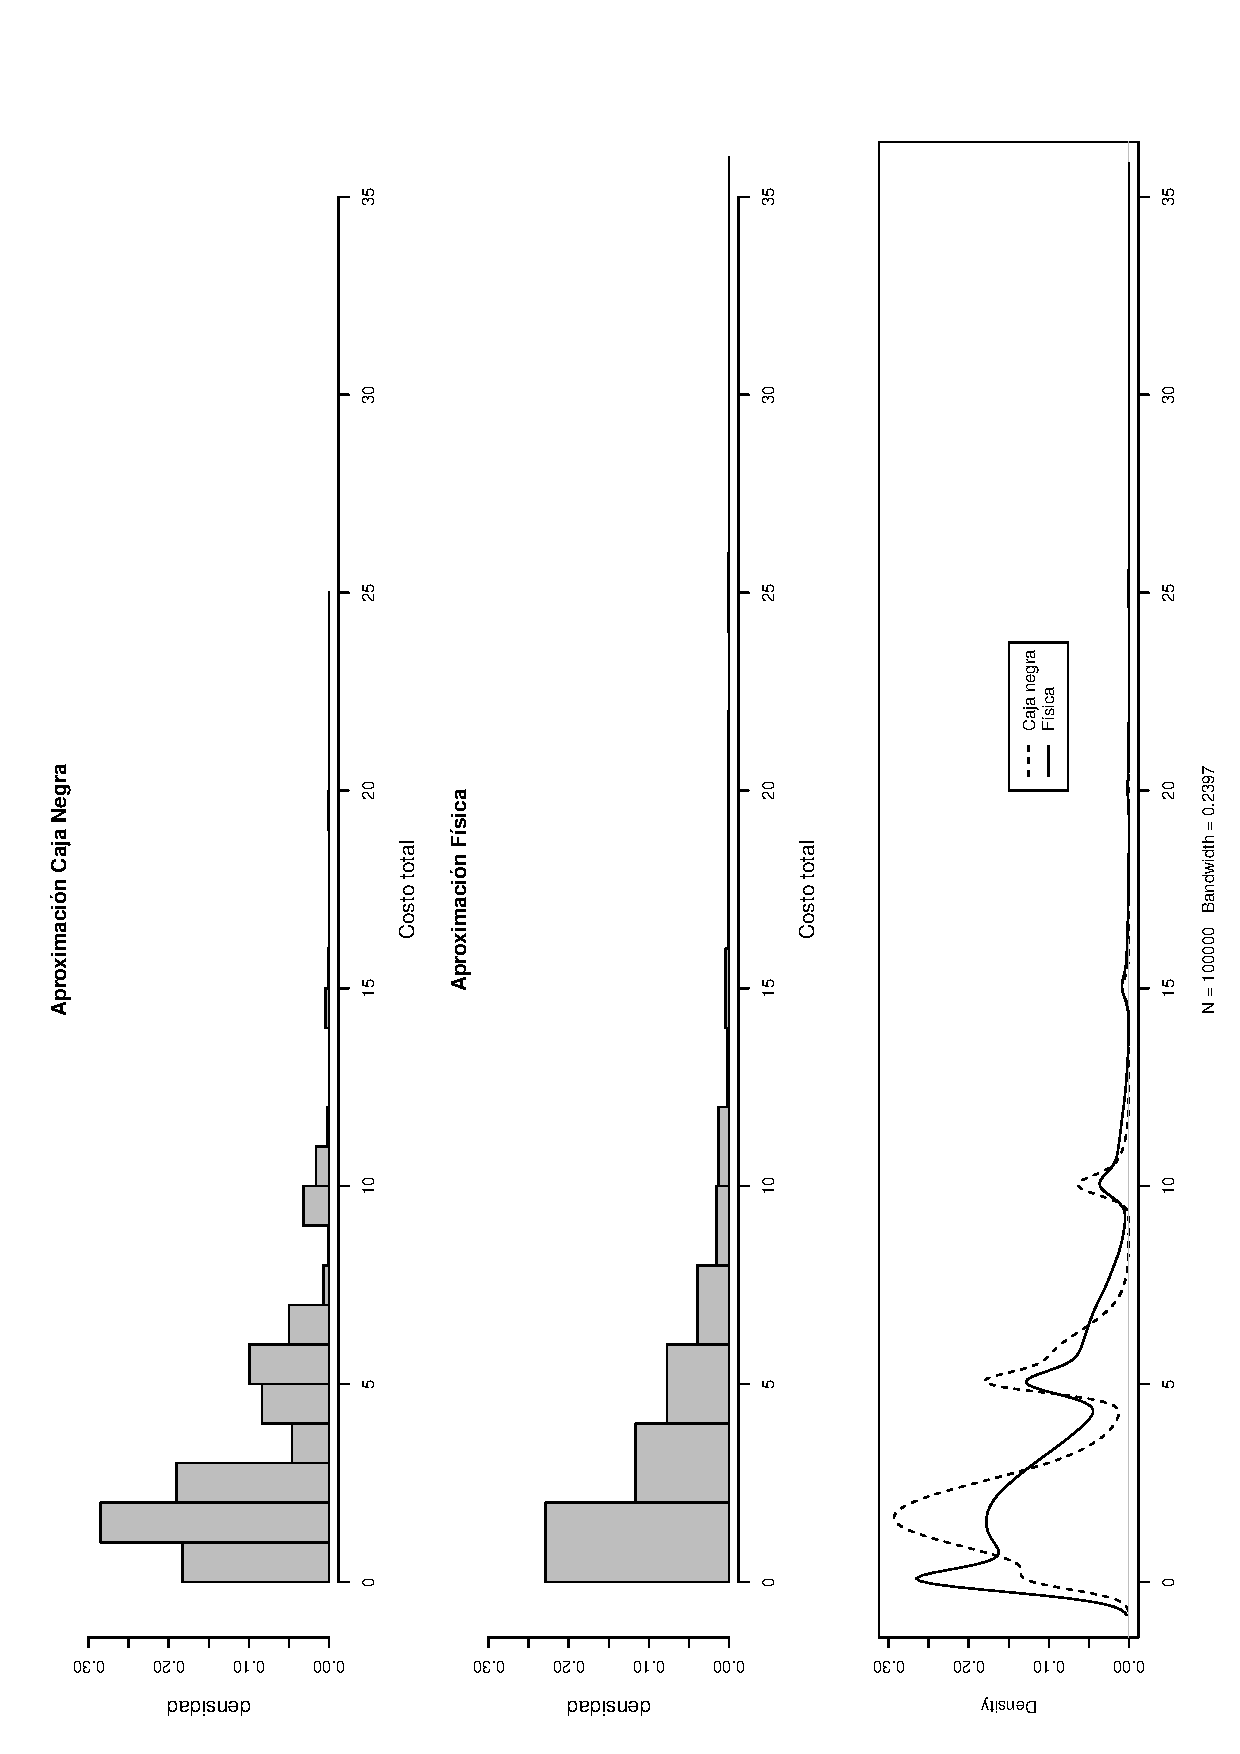
\includegraphics[scale=0.4, angle=-90]{Kap3/Fig_Cap3/Costo_Total}
\caption{Histograma de costos totales de garant\'{\i}a. Pol\'{\i}tica PRW.} \label{Fi}
\end{figure}

\subsection*{Acerca de las notas al pie}

En general se evitar\'{a} el uso de llamadas fuera del texto principal para introducir aclaraciones o complementos. Pero en la situaci\'{o}n eventual de que esto se necesite (algo altamente improbable) estas llamadas deben hacerse con un nota al pie\footnote{ Solo en caso de necesidad extrema, las notas se usar\'{\i}an como ``notas al pie". Se utilizan para explicar, comentar o hacer referencia al texto de un documento, as\'{\i} como para introducir comentarios detallados. \emph{Las notas al pie no se usan en este informe final de Trabajo de Grado para introducir referencias bibliogr\'{a}ficas}.}.\\

La fuente documental se debe escribir al final de la figura con los elementos de la referencia (de acuerdo con las normas seleccionadas) y no como pie de p\'{a}gina. \\

\section{Presentaci\'{o}n y citaci\'{o}n de tablas}

Para la edici\'{o}n de tablas, cada columna debe llevar su t\'{\i}tulo; la primera palabra se debe escribir con may\'{u}scula inicial y preferiblemente sin abreviaturas. En las tablas y cuadros, los t\'{\i}tulos y datos se deben ubicar entre l\'{\i}neas horizontales y verticales cerradas (como se realiza en esta plantilla).\\

La numeraci\'{o}n de las tablas se realiza de la misma manera que las figuras o ilustraciones, a lo largo de todo el texto. Deben llevar un t\'{\i}tulo breve, que concreta el contenido de la tabla; \'{e}ste se debe escribir en la parte superior de la misma. Para la presentaci\'{o}n de cuadros, se deben seguir las indicaciones dadas para las tablas.\\

Un ejemplo para la presentaci\'{o}n y citaci\'{o}n de tablas (citaci\'{o}n indirecta), se presenta a continuaci\'{o}n:\\
\\
Los resultados de la prueba chi-cuadrado sugieren fuerte evidencia para rechazar la hip\'{o}tesis nula de igualdad distribucional. Ver Tabla \ref{Ta} \\

\begin{table}[htbp]
\centering
\caption{Prueba Chi-cuadrado de igualdad distribucional entre aproximaci\'{o}n caja negra y aproximaci\'{o}n f\'{\i}sica. Pol\'{\i}tica FRW.} \label{Ta}
\begin{tabular}{|c|c|c|c|} \hline              
  & $\chi^{2}$  & df   & valor-p  \\\hline
costo falla I & 12379.12 & 6 & $< 2.2 \times 10^{-16}$ \\\hline
costo falla II & 5893.437 & 17 & $< 2.2 \times 10^{-16}$ \\\hline
costos total & 10700.75 & 26 & $< 2.2 \times 10^{-16}$  \\\hline
\end{tabular}%
\end{table}

\textbf{NOTA:} en el caso en que el contenido de la tabla sea muy extenso, se puede cambiar el tama\~{n}o de la letra, siempre y cuando \'{e}sta sea visible por el lector.\\

\subsection{Consideraciones adicionales para el manejo de figuras, tablas y ecuaciones}
Cuando una tabla, cuadro o figura ocupa m\'{a}s de una p\'{a}gina, se debe repetir su identificaci\'{o}n num\'{e}rica, seguida por la palabra continuaci\'{o}n.\\

Adicionalmente los encabezados de las columnas se deben repetir en todas las p\'{a}ginas despu\'{e}s de la primera.\\

Los anteriores lineamientos se contemplan en la presente plantilla.\\

\begin{itemize}
\item Presentaci\'{o}n y citaci\'{o}n de ecuaciones.
\end{itemize}

La citaci\'{o}n de ecuaciones, en caso que se presenten, debe hacerse como lo sugiere esta plantilla. Todas las ecuaciones deben estar numeradas y citadas detro del texto.\\

Para el manejo de cifras se debe seleccionar la norma seg\'{u}n el \'{a}rea de conocimiento del trabajo de grado. \\

\begin{equation}\label{procFRW_bb}
Z_{w}^{FRW}= \sum_{j=1}^{\eta} \left( c^{I} N_{T^{II}_{j}}^{I} + c^{II}\right) -\left( c^{I} N_{T^{II}_{\eta}}^{I} + c^{II} \right) + c^{I} N_{w}^{I}
\end{equation}

y el valor esperado del proceso de costo (\ref{procFRW_bb}) se encuentra dado por,

\begin{equation}\label{esperanza_FRW_bb}
E\left( Z_{w}^{FRW}\right) = E\left[ \sum_{j=1}^{\eta} \left(c^{I} N_{T^{II}_{j}}^{I} + c^{II}\right) - \left(c^{I} N_{T^{II}_{\eta}}^{I} + c^{II}\right)    \right]   + E \left[  c^{I} N_{w}^{I}\right] 
\end{equation}

Para obtener la expresi\'{o}n del valor esperado del proceso de costo $Z_{w}^{FRW}$ en (\ref{esperanza_FRW_bb}) se realiza el c\'{a}lculo de la esperanza para cada uno de los t\'{e}rminos que componen la expresi\'{o}n.
%\chapter{Normatividad sobre el trabajo de grado}

A continuaci\'{o}n se presentan los requisitos necesarios para la realizaci\'{o}n del Trabajo de Grado en el Programa Acad\'{e}mico de Estad\'{\i}stica basados en la reglamentaci\'{o}n establecida por el Consejo Superior de la Universidad del Valle.

\section{Reglamento estudiantil}

El Acuerdo 009 de 1997 emanado por el Consejo Superior
\begin{itemize}
\item Reglamenta las actividades acad\'{e}micas de los estudiantes regulares pertenecientes a los Progr\'{a}mas Acad\'{e}micos de Pregrado.

\item En el cap\'{\i}tulo XIV reglamenta los trabajos de grado
\end{itemize}

\section{De los trabajos de grado}

El Acuerdo No. 009 del 13 de noviembre de 1997, emanado por el Consejo Superior establece en su art\'{\i}culo 90 que:\\

\textbf{Art\'{\i}culo 90}: En todos los Programas Acad\'{e}micos de la Universidad,
se exigir\'{a} como requisito parcial para la obtenci\'{o}n del t\'{\i}tulo, un Trabajo de Grado, el cual podr\'{a} tener diferentes modalidades: Monograf\'{\i}a,
Proyecto, Pasant\'{\i}a, Pr\'{a}ctica, Ensayo, Traducci\'{o}n Cr\'{\i}tica u otras
aprobadas por el Consejo Acad\'{e}mico. Cada modalidad depender\'{a} de los objetivos del Programa Acad\'{e}mico, del perfil profesional del egresado, del nivel de exigencia que el Programa Acad\'{e}mico defina para esta asignatura y de los intereses del estudiante.\\\\ El Trabajo de Grado puede orientarse a la sistematizaci\'{o}n de conocimientos, a la formulaci\'{o}n y soluci\'{o}n de problemas de investigaci\'{o}n, a la definici\'{o}n y dise\~{n}o de proyectos destinados a la aclaraci\'{o}n de aspectos pr\'{a}cticos de diferente orden, al dise\~{n}o, realizaci\'{o}n y evaluaci\'{o}n de proyectos de intervenci\'{o}n en el \'{a}rea profesional o a la actividad pr\'{a}ctica en la soluci\'{o}n de problemas en las
respectivas disciplina.\\\\\
Le corresponde al Consejo de Facultad definir aquellos aspectos comunes de reglamentaci\'{o}n de sus Programas Acad\'{e}micos.\\


\subsection{Reglamentaciones por facultad, Distinciones}

\begin{itemize}
\item \textbf{ Par\'{a}grafo 1.} Los Comit\'{e}s de Curr\'{\i}culo de las diferentes
Facultades, definir\'{a}n aquellos aspectos de la reglamentaci\'{o}n
comunes a sus Programas y, con base en ellos, cada Programa
Acad\'{e}mico establecer\'{a} su reglamento espec\'{\i}fico.

\item \textbf{Par\'{a}grafo 2.} En la Universidad se calificar\'{a}n como ``meritorios'' \'{o} ``laureados'', aquellos Trabajos de Grado que, de acuerdo con las
reglamentaciones de las respectivas Facultades, alcancen los
niveles de excelencia requeridos para la asignaci\'{o}n de tales
calificaciones.
\end{itemize}

\subsection{Duraci\'{o}n}
\textbf{Art\'{\i}culo 91.} Todo estudiante tendr\'{a} un plazo hasta de dos (2)
semestres para concluir su Trabajo de Grado. Este plazo se
contabilizar\'{a} a partir de la primera matr\'{\i}cula de la \emph{asignatura} ``Trabajo
de Grado''.
\begin{itemize}
\item\textbf{ Par\'{a}grafo.} Por causa debidamente justificada, el Comit\'{e} del
Programa Acad\'{e}mico podr\'{a} prorrogar el plazo se\~{n}alado hasta por
dos (2) semestres.
\item\textbf{ Art\'{\i}culo 92.} En los dos (2) primeros semestres de que habla el
Art\'{\i}culo anterior, el estudiante matricular\'{a} la asignatura ``Trabajo
de Grado'', o su equivalente, y en los subsiguientes, la asignatura
``Continuaci\'{o}n del Trabajo de Grado''.
\end{itemize}

\subsection{Exenci\'{o}n de matr\'{\i}cula durante la continuaci\'{o}n de trabajo de
grado}
\textbf{Par\'{a}grafo} Si el estudiante matricula \'{u}nicamente la asignatura
``Continuaci\'{o}n del Trabajo de Grado'', podr\'{a} cancelar el valor
correspondiente al 25\% del salario m\'{\i}nimo mensual vigente por
concepto de matr\'{\i}cula financiera. El estudiante que deba matricular
otras asignaturas o \'{e}l que encontr\'{a}ndose a paz y salvo con su
Programa Acad\'{e}mico desee tomar otras asignaturas, deber\'{a} cancelar
el valor total de la matr\'{\i}cula. El Director del Programa velar\'{a} por el
cumplimiento de esta norma y la secci\'{o}n de Registro Acad\'{e}mico
verificar\'{a} si esto se efectu\'{o}.

\subsection{Condiciones de grado}
\textbf{Art\'{\i}culo 93}. Para la obtenci\'{o}n del grado, el estudiante debe
matricular en forma sucesiva los semestres que sean necesarios para
la culminaci\'{o}n, presentaci\'{o}n, sustentaci\'{o}n y aprobaci\'{o}n del Trabajo de
Grado.
\begin{itemize}

\item \textbf{Par\'{a}grafo 1.} Si el estudiante ha cumplido con todos los requisitos
para grado, podr\'{a} recibir su t\'{\i}tulo en las fechas previstas para
ello, aunque no haya finalizado el per\'{\i}odo acad\'{e}mico en el cual
se encuentra matriculado.

\item \textbf{Par\'{a}grafo 2.} Si el estudiante no realiza la matr\'{\i}cula de manera
sucesiva, deber\'{a} solicitar reingreso.

\item \textbf{Par\'{a}grafo 3.} Si el estudiante no present\'{o} el Trabajo de Grado en
los plazos establecidos o si el resultado final del Trabajo de Grado
no es aprobatorio, podr\'{a} solicitar su reingreso al Programa
Acad\'{e}mico. En estos casos, el Comit\'{e} de Programa Acad\'{e}mico
definir\'{a} cu\'{a}les asignaturas adicionales al Trabajo de Grado
deber\'{a} matricular.

\item \textbf{Par\'{a}grafo 4.} Si por segunda vez se vence el plazo m\'{a}ximo
previsto de cuatro (4) semestres y no se ha aprobado el Trabajo
de Grado, el estudiante pierde el derecho a optar por el t\'{\i}tulo y el
Director de Programa Acad\'{e}mico notificar\'{a} a las instancias
respectivas la calificaci\'{o}n de ``no aprob\'{o}''.
\end{itemize}


\section{Reglamentaci\'{o}n en la Facultad de Ingenier\'{\i}a: Resoluci\'{o}n No 074 de junio 21 de 2011}

\subsection{Resoluci\'{o}n No 074 de junio 21 de 2011, Consejo de Facultad}
Reglamenta el Trabajo de Grado para la Facultad de Ingenier\'{\i}a.
\begin{itemize}
\item \textbf{Art\'{\i}culo 2.} El Trabajo de Grado podr\'{a} tener diferentes
modalidades tales como Monograf\'{\i}a, Trabajo de investigaci\'{o}n e
innovaci\'{o}n, Pasant\'{\i}as, Creaci\'{o}n de empresa o Cursos en
postgrado.

\item \textbf{Par\'{a}grafo 1.} Los Comit\'{e}s de Programa Acad\'{e}mico reglamentar\'{a}n y definir\'{a}n, con base en la estructura curricular y prop\'{o}sitos de
formaci\'{o}n de los programas acad\'{e}micos, las modalidades de Trabajo de Grado a las que pueden optar sus estudiantes.
\end{itemize}

\subsection{Trabajo de Investigaci\'{o}n e innovaci\'{o}n}
\begin{itemize}
\item Hasta la fecha la modalidad aceptada en Estad\'{\i}stica es la
denominada ``Trabajo de investigaci\'{o}n e Innovaci\'{o}n'', que se
define as\'{\i}:
\item Presentaci\'{o}n formal del resultado de un proceso de exploraci\'{o}n,
descripci\'{o}n, correlaci\'{o}n, explicaci\'{o}n o compresi\'{o}n de sujetos,
objetos o fen\'{o}menos. Debe seguir la metodolog\'{\i}a cient\'{\i}fica y
cubrir las diversas etapas del proceso de investigaci\'{o}n, para crear
nuevo conocimiento o plantear soluciones factibles. Esta actividad
debe adelantarse con el aval de un grupo de investigaci\'{o}n o en el
marco de un proyecto en particular, buscando una efectiva
orientaci\'{o}n del trabajo.
\end{itemize}


\subsection{El informe final}
\textbf{Par\'{a}grafo 2}. Todas las modalidades de Trabajo de Grado concluyen
en un informe escrito y una sustentaci\'{o}n p\'{u}blica conforme a lo
establecido por esta Resoluci\'{o}n exceptuando la excelencia
acad\'{e}mica.

\subsection{Asignaturas que conforman el trabajo de grado en programas de
ingenier\'{\i}a}

\textbf{Art\'{\i}culo 6.} El Trabajo de Grado para un Programa Acad\'{e}mico en
Ingenier\'{\i}a tendr\'{a} m\'{\i}nimo siete (7) cr\'{e}ditos distribuidos en tres (3)
asignaturas, as\'{\i}:
\begin{itemize}
\item Anteproyecto o su equivalente Un (1) Cr\'{e}dito m\'{\i}nimo
\item Trabajo de Grado I o su equivalente Dos (2) Cr\'{e}ditos m\'{\i}nimo
\item Trabajo de Grado II o su equivalente Cuatro (4) Cr\'{e}ditos m\'{\i}nimo
\end{itemize}

\subsection{Asignaturas que conforman el trabajo de grado en el programa
acad\'{e}mico de Estad\'{\i}stica}

La Resoluci\'{o}n No. 079 del 6 de Junio del 2002 establece:\\

\textbf{Art\'{\i}culo 6.} El programa acad\'{e}mico de Estad\'{\i}stica, c\'{o}digo 3752, tiene
una duraci\'{o}n de 10 semestres, modalidad presencial y jornada diurna
y exige como m\'{\i}nimo 166 cr\'{e}ditos.
\begin{itemize}
\item\textbf{ Par\'{a}grafo 7.} El Trabajo de Grado est\'{a} conformado por tres
asignaturas, Estad\'{\i}stica Aplicada IV, Trabajo de Grado I y Trabajo
de Grado II. De estos, el curso de Estad\'{\i}stica Aplicada IV est\'{a}
reservado para que en el desarrollo del mismo se realice el
anteproyecto del Trabajo de Grado.
\end{itemize}

\section{Distinciones en Ingenier\'{\i}a: Resoluci\'{o}n No 085 de Mayo 26 de 2009}

\subsection{Resoluci\'{o}n No 085 de 2009, Consejo de Facultad}
Establece los criterios y el procedimiento para la calificaci\'{o}n de
Meritorio o Laureado de un Trabajo de Grado de Pregrado en la
Facultad de Ingenier\'{\i}a.

\begin{itemize} 
\item \textbf{Art\'{\i}culo 2.} Para optar a la calificaci\'{o}n de Meritorio o Laureado,
son requisitos indispensables que el Trabajo de Grado se haya
ejecutado en el tiempo aprobado en el cronograma del
anteproyecto, sin superar lo establecido en la estructura curricular
del programa para la terminaci\'{o}n del Trabajo de Grado, con las
excepciones de fuerza mayor debidamente certificadas y
autorizadas por el Comit\'{e} de Programa, y que el Trabajo de Grado
haya obtenido como m\'{\i}nimo la siguiente calificaci\'{o}n num\'{e}rica:
\begin{itemize}
\item Trabajo de Grado Meritorio 4.5 (Cuatro punto cinco)
\item Trabajo de Grado Laureado 5.0 (Cinco punto cero)
\end{itemize}
\end{itemize}

\section{Recomendaciones}
\begin{itemize}
\item El trabajo de grado no debe exceder un tama\~{n}o m\'{a}ximo de 80
p\'{a}ginas (Resoluci\'{o}n 074 de 2011), incluyendo anexos.
\item El anteproyecto de grado, en consecuencia, no debe exceder un
tama\~{n}o m\'{a}ximo de 20 p\'{a}ginas, incluyendo anexos.
\item El periodo de ejecuci\'{o}n del proyecto es de m\'{a}ximo un a\~{n}o.
\end{itemize}
%\chapter{Cap\'{\i}tulo...}
Se deben incluir tantos cap\'{\i}tulos como se requieran; sin embargo, se recomienda que el Trabajo de Grado tenga un m\'{\i}nimo 3 cap\'{\i}tulos y m\'{a}ximo de 6 cap\'{\i}tulos (incluyendo las conclusiones).\\ 
\chapter{Conclusion}
Las conclusiones constituyen un cap\'{\i}tulo independiente y presentan, en forma l\'{o}gica, los resultados del trabajo de grado. Las conclusiones deben ser la respuesta a los objetivos o prop\'{o}sitos planteados. Se deben titular con la palabra conclusiones en el mismo formato de los t\'{\i}tulos de los cap\'{\i}tulos anteriores (T\'{\i}tulos primer nivel), precedida por el numeral correspondiente (seg\'{u}n la presente plantilla).



\begin{appendix}
\chapter{Appendix}\label{AnexoA}
Los Anexos son documentos o elementos que complementan el cuerpo de la tesis o trabajo de investigaci\'{o}n y que se relacionan, directa o indirectamente, con el trabajo de grado, tales como acetatos, cd, normas, etc.

%\chapter{Anexo: Nombrar el anexo B de acuerdo con su contenido}
%A final del documento es opcional incluir \'{\i}ndices o glosarios. \'{E}stos son listas detalladas y especializadas de los t\'{e}rminos, nombres, autores, temas, etc., que aparecen en el mismo. Sirven para facilitar su localizaci\'{o}n en el texto. Los \'{\i}ndices pueden ser alfab\'{e}ticos, cronol\'{o}gicos, num\'{e}ricos, anal\'{\i}ticos, entre otros. Luego de cada palabra, t\'{e}rmino, etc., se pone coma y el n\'{u}mero de la p\'{a}gina donde aparece esta informaci\'{o}n.\\
\end{appendix}

\addcontentsline{toc}{chapter}{\numberline{}References}
\bibliographystyle{agsm}
\bibliography{BiblioPAE}
\end{document}